%%%%%%%%%%%%%%
%% Run LaTeX on this file several times to get Table of Contents,
%% cross-references, and citations.

%% If you have font problems, you may edit the w-bookps.sty file
%% to customize the font names to match those on your system.

%% w-bksamp.tex. Current Version: Feb 16, 2012
%%%%%%%%%%%%%%%%%%%%%%%%%%%%%%%%%%%%%%%%%%%%%%%%%%%%%%%%%%%%%%%%
%
%  Sample file for
%  Wiley Book Style, Design No.: SD 001B, 7x10
%  Wiley Book Style, Design No.: SD 004B, 6x9
%
%
%  Prepared by Amy Hendrickson, TeXnology Inc.
%  http://www.texnology.com
%%%%%%%%%%%%%%%%%%%%%%%%%%%%%%%%%%%%%%%%%%%%%%%%%%%%%%%%%%%%%%%%

%%%%%%%%%%%%%
% 7x10
%\documentclass{wileySev}

% 6x9
\documentclass{wileySix}

\usepackage{graphicx}

%%%%%%%
%% for times math: However, this package disables bold math (!)
%% \mathbf{x} will still work, but you will not have bold math
%% in section heads or chapter titles. If you don't use math
%% in those environments, mathptmx might be a good choice.

% \usepackage{mathptmx}

% For PostScript text
\usepackage{w-bookps}

%%%%%%%%%%%%%%%%%%%%%%%%%%%%%%%%%%%%%%%%%%%%%%%%%%%%%%%%%%%%%%%%
%% Other packages you might want to use:

% for chapter bibliography made with BibTeX
% \usepackage{chapterbib}

% for multiple indices
% \usepackage{multind}

% for answers to problems
% \usepackage{answers}

%%%%%%%%%%%%%%%%%%%%%%%%%%%%%%
%% Change options here if you want:
%%
%% How many levels of section head would you like numbered?
%% 0= no section numbers, 1= section, 2= subsection, 3= subsubsection
%%==>>
\setcounter{secnumdepth}{3}

%% How many levels of section head would you like to appear in the
%% Table of Contents?
%% 0= chapter titles, 1= section titles, 2= subsection titles, 
%% 3= subsubsection titles.
%%==>>
\setcounter{tocdepth}{2}

%% Cropmarks? good for final page makeup
%% \docropmarks

%%%%%%%%%%%%%%%%%%%%%%%%%%%%%%
%
% DRAFT
%
% Uncomment to get double spacing between lines, current date and time
% printed at bottom of page.
% \draft
% (If you want to keep tables from becoming double spaced also uncomment
% this):
% \renewcommand{\arraystretch}{0.6}
%%%%%%%%%%%%%%%%%%%%%%%%%%%%%%

%%%%%%% Demo of section head containing sample macro:
%% To get a macro to expand correctly in a section head, with upper and
%% lower case math, put the definition and set the box 
%% before \begin{document}, so that when it appears in the 
%% table of contents it will also work:

\newcommand{\VT}[1]{\ensuremath{{V_{T#1}}}}

%% use a box to expand the macro before we put it into the section head:

\newbox\sectsavebox
\setbox\sectsavebox=\hbox{\boldmath\VT{xyz}}

%%%%%%%%%%%%%%%%% End Demo


\begin{document}


\booktitle{Survey Methodology}
\subtitle{This is the Subtitle}

\authors{Robert M. Groves\\
\affil{Universitat de les Illes Balears}
Floyd J. Fowler, Jr.\\
\affil{University of New Mexico}
}

\offprintinfo{Survey Methodology, Second Edition}{Robert M. Groves}

%% Can use \\ if title, and edition are too wide, ie,
%% \offprintinfo{Survey Methodology,\\ Second Edition}{Robert M. Groves}

%%%%%%%%%%%%%%%%%%%%%%%%%%%%%%
%% 
\halftitlepage

\titlepage


\begin{copyrightpage}{2007}
Survey Methodology / Robert M. Groves . . . [et al.].
\       p. cm.---(Wiley series in survey methodology)
\    ``Wiley-Interscience."
\    Includes bibliographical references and index.
\    ISBN 0-471-48348-6 (pbk.)
\    1. Surveys---Methodology.  2. Social 
\  sciences---Research---Statistical methods.  I. Groves, Robert M.  II. %
Series.\\

HA31.2.S873 2007
001.4'33---dc22                                             2004044064
\end{copyrightpage}

\dedication{To my parents}

\begin{contributors}
\name{Masayki Abe,} Fujitsu Laboratories Ltd., Fujitsu Limited, Atsugi,
Japan

\name{L. A. Akers,} Center for Solid State Electronics Research, Arizona
State University, Tempe, Arizona

\name{G. H. Bernstein,} Department of Electrical and
Computer Engineering, University of Notre Dame, Notre Dame, South Bend, 
Indiana; formerly of
Center for Solid State Electronics Research, Arizona
State University, Tempe, Arizona 
\end{contributors}

\contentsinbrief
\tableofcontents
\listoffigures
\listoftables


\begin{foreword}
This is the foreword to the book.
\end{foreword}

\begin{preface}
This is an example preface.
This is an example preface.
This is an example preface.
This is an example preface.

\prefaceauthor{R. K. Watts}
\where{Durham, North Carolina\\
September, 2007}

\end{preface}


\begin{acknowledgments}
From Dr.~Jay Young, consultant from Silver Spring, Maryland, I received
the initial push to even consider writing this book. Jay was a constant
``peer reader'' and very welcome advisor durying this year-long process.


To all these wonderful people I owe a deep sense of gratitude especially now
that this project has been completed.
\authorinitials{G. T. S.}
\end{acknowledgments}

\begin{acronyms}
\acro{ACGIH}{American Conference of Governmental Industrial Hygienists}
\acro{AEC}{Atomic Energy Commission}
\acro{OSHA}{Occupational Health and Safety Commission}
\acro{SAMA}{Scientific Apparatus Makers Association}
\end{acronyms}

\begin{glossary}
\term{NormGibbs}Draw a sample from a posterior distribution
of data with an unknown mean and variance using Gibbs sampling.

\term{pNull}Test a one sided hypothesis from a numberically
specified posterior CDF or from a sample from the posterior

\term{sintegral}A numerical integration using Simpson's rule
\end{glossary}

\begin{symbols}
\term{A}Amplitude

\term{\hbox{\&}}Propositional logic symbol 

\term{a}Filter Coefficient

\bigskip

\term{\mathcal{B}}Number of Beats
\end{symbols}

\begin{introduction}

%% optional, but if you want to list author:

\introauthor{Catherine Clark, PhD.}
{Harvard School of Public Health\\
Boston, MA, USA}

The era of modern \index{microelectronics}\index{microelectronics!modern} 
began in 1958 with the invention of the
integrated circuit by J.~S.~Kilby
 of Texas Instruments \cite{kilby}.
His first chip is shown in Fig.~I. For comparison,
Fig.~I.2 shows a modern microprocessor chip, \cite{beren}.


This is the introduction.
This is the introduction.
This is the introduction.
This is the introduction.
This is the introduction.
This is the introduction.

\begin{equation}
ABC {\cal DEF} \alpha\beta\Gamma\Delta\sum^{abc}_{def}
\end{equation}


\begin{chapreferences}{3.}
\bibitem{zkilby}J. S. Kilby,
``Invention of the Integrated Circuit,'' {\it IEEE Trans. Electron Devices,}
{\bf ED-23,} 648 (1976).

\bibitem{zhamming}R. W. Hamming,
                 {\it Numerical Methods for Scientists and 
                 Engineers}, Chapter N-1, McGraw-Hill, 
                 New York, 1962.

\bibitem{zHu}J. Lee, K. Mayaram, and C. Hu, ``A Theoretical
               Study of Gate/Drain Offset in LDD MOSFETs''
                     {\it IEEE Electron Device Lett.,} {\bf EDL-7}(3). 152 
                     (1986).
\end{chapreferences}
\end{introduction}


\part[Submicron Semiconductor Manufacture]
{Submicron Semiconductor\\ Manufacture}


\chapter[The Submicrometer Silicon MOSFET]
{The Submicrometer\\ Silicon MOSFET}


\prologue{The sheer volumne of answers can often stifle insight...The purpose
of computing\index{computing!the purpose} is insight, not numbers.}
{Hamming \cite{hamming}}


\section{Here is a normal section}
Here is some text.

\subsection{This is the subsection}
Here is some normal text.
Here is some normal text.
Here is some normal text.
Here is some normal text.
Here is some normal text.
Here is some normal text.
Here is some normal text.
Here is some normal text.
Here is some normal text.
Here is some normal text.
Here is some normal text.


\subsubsection{This is the subsubsection}
Here is some text after the subsubsection.
Here is some text after the subsubsection.
Here is some text after the subsubsection.
Here is some text after the subsubsection.

\paragraph{This is the paragraph}
Here is some normal text.
Here is some normal text.
Here is some normal text.
Here is some normal text.

\section{Tips On Special Section Heads}
Here are some things you can do for a special
section head.

\section[This Version of Section Head will be sent Contents]
{Break Long Section heads\\ with double backslash}
Here is some normal text.
Here is some normal text.
Here is some normal text.

 \section[This show how to explicitly break lines
\string\hfill\string\break\space in Table of Contents]
{Here is a Section Title}
See this section head for information on how to explicitly break lines in
table of contents.

\section{How to get \lowercase{lower case} in section head: \lowercase{$p$}$H$}
Here is some normal text.
Here is some normal text.
Here is some normal text.

\section{How to use a macro that has both upper and lower case parts: 
\copy\sectsavebox}
See the top of this file where the definition and box were set.

%% Sending different version of section to running head, 
%% so that the size of math is correct in running head:
\markright{Sample macro \VT{\lowercase{xyz}} sent to running head}

\section{Equation}

For optimal vertical spacing, no blank lines before or after
equations
\begin{equation}
\alpha\beta\Gamma\Delta
\end{equation}
as you see here.


\chapter{First Edited Book Sample Chapter Title}
\chapterauthors{G. Alvarez and R. K. Watts
\chapteraffil{Carnegie Mellon University, Pittsburgh, Pennsylvania}
}

\section{Here is a normal section}
Here is some text.


\chapter{Second Edited Book Sample Chapter Title}
\chapterauthors{George Smeal, Ph.D.\affilmark{1}, Sally Smith,
M.D.\affilmark{2} and Stanley Kubrick\affilmark{1}
\chapteraffil{\affilmark{1}AT\&T Bell Laboratories
Murray Hill, New Jersey\\
\affilmark{2}Harvard Medical School,
Boston, Massachusetts}
}

\section{Sample Section}
Here is some sample text.

\newpage

\section{Example, Figure and Tables}
\vskip6pt
\begin{example}[Optional Example Name]
Use Black's law [Equation (6.3)] to estimate the reduction in useful product
life if a metal line is initially run at 55$^\circ$C at a maximum line
current density.
\end{example}


\begin{figure}[ht]
illustration here
%\centerline{\includegraphics[width=.5\textwidth]{filename}}
\caption{Short figure caption.}
\end{figure}

\begin{figure}[ht]
\vskip2pt
\caption{Oscillograph for  memory address access operations,
showing 500 ps
address access time and superimposed signals
of address access in 1 kbit
memory plane.}
\end{figure}

\begin{table}[ht]
\caption{Small Table}
\centering
\begin{tabular}{cccc}
\hline
one&two&three&four\\
\hline
C&D&E&F\\
\hline
\end{tabular}
\end{table}



\begin{table}[ht]
\caption{Effects of the two types of $\alpha\beta\sum^A_B$ scaling proposed by Dennard \newline
and
co-workers$^{a,b}$}
\begin{tabular*}{\textwidth}{@{\extracolsep{\fill}}lcc}
\hline
Parameter& $\kappa$ Scaling & $\kappa$, $\lambda$ Scaling\cr
\hline
Dimension&$\kappa^{-1}$&$\lambda^{-1}$\cr
Voltage&$\kappa^{-1}$&$\kappa^{-1}$\cr
Currant&$\kappa^{-1}$&$\lambda/\kappa^{2}$\cr
Dopant Concentration&$\kappa$&$\lambda^2/\kappa$\cr
\hline
\end{tabular*}
\begin{tablenotes}
$^a$Refs.~19 and 20.

$^b\kappa, \lambda>1$.
\end{tablenotes}
\end{table}

\subsection{Side by Side Tables and Figures}

\begin{figure}[ht]
\sidebyside{
Space for figure...
\caption{This caption will go on the left side of
the page. It is the initial caption of two side-by-side captions.}
}
{
Space for second figure...
\caption{This caption will go on the right side of
the page. It is the second of two side-by-side captions.}
}
\end{figure}


The command \verb+\sidebyside{}{}+ works similarly for tables:

 \begin{table}[ht]
 \sidebyside{
\caption{Table Caption} 
\begin{tabular}{cccc}
one&two&three&four\\
a &little&sample&table
\end{tabular}
}
 {
\caption{Table Caption}
\begin{tabular}{cccc}
A&B&C&D\\
a &second little& sample&table
\end{tabular}
}
 \end{table}


When using \verb+\sidebyside+, one must
use the cross referencing command \verb+\label{}+ after and  {\it outside} 
 of \verb+\caption{}+:

\begin{verbatim}
 \begin{table} 
 \sidebyside{\caption{Table Caption}\label{tab1}
 first table}
 {\caption{Table Caption}\label{tab2} second table}
 \end{table}
\end{verbatim}
 or,
\begin{verbatim}
 \begin{figure} 
 \sidebyside{\vskip<dimen>\caption{fig caption}\label{fig1}}
 {\vskip<dimen>\caption{fig caption}\label{fig2}}
 \end{figure}
\end{verbatim}





\section{Algorithm}
This is a sample algorithm.

\begin{algorithm}
{\bf state\_transition algorithm} $\{$
\        for each neuron $j\in\{0,1,\ldots,M-1\}$
\        $\{$   
\            calculate the weighted sum $S_j$ using Eq. (6);
\            if ($S_j>t_j$)
\                    $\{$turn ON neuron; $Y_1=+1\}$   
\            else if ($S_j<t_j$)
\                    $\{$turn OFF neuron; $Y_1=-1\}$   
\            else
\                    $\{$no change in neuron state; $y_j$ remains %
unchanged;$\}$ 
\        $\}$   
$\}$   
\end{algorithm}

Here is some normal text.
Here is some normal text.
Here is some normal text.
Here is some normal text.
Here is some normal text.
Here is some normal text.
Here is some normal text.
Here is some normal text.
Here is some normal text.
Here is some normal text.
Here is some normal text.
Here is some normal text.
Here is some normal text.
Here is some normal text.


\begin{quote}
This is a sample of extract or quotation.
This is a sample of extract or quotation.
This is a sample of extract or quotation.
\end{quote}

\begin{enumerate}
\item
This is the first item in the numbered list.

\item
This is the second item in the numbered list.
This is the second item in the numbered list.
This is the second item in the numbered list.
\end{enumerate}

\begin{itemize}
\item
This is the first item in the itemized list.

\item
This is the first item in the itemized list.
This is the first item in the itemized list.
This is the first item in the itemized list.
\end{itemize}

\begin{itemize}
\item[]
This is the first item in the itemized list.

\item[]
This is the first item in the itemized list.
This is the first item in the itemized list.
This is the first item in the itemized list.
\end{itemize}

\begin{problems}
\prob
For Hooker's data, Problem 1.2, use the Box and Cox and Atkinson procedures to determine a appropriate transformation of PRES
in the regression of PRES on TEMP. find $\hat\lambda$, $\tilde\lambda$,
the score test, and the added variable plot for the score. 
Summarize the results.

\prob
The following data were collected in a study of the effect of dissolved sulfur
on the surface tension of liquid copper (Baes and Killogg, 1953).

{\centering
\vskip6pt
\begin{tabular}{rlcc}
\hline
&&\multicolumn2c{$Y$= Decrease in Surface Tension}\\
\multicolumn2c{$x$ = Weight \% sulfur}
&\multicolumn2c{(dynes/cm), two Replicates}\\
\hline
0.&034&301&316\\
0.&093&430&422\\
0.&30&593&586\\
\hline
\end{tabular}
\vskip6pt
}


\subprob
Find the transformations of $X$ and $Y$ sot that in the transformed scale 
the regression is linear.

\subprob
Assuming that $X$ is transformed to $\ln(X)$, which choice of $Y$ gives 
better results,
$Y$ or $\ln(Y)$? (Sclove, 1972).

\sidebysidesubprob{In the case of $\alpha_1$?}{In the case of $\alpha_2$?}

\prob
Examine the Longley data, Problem 3.3, for applicability of assumptions of the
linear model.

\sidebysideprob{In the case of $\Gamma_1$?}{In the case of $\Gamma_2$?}

\end{problems}


\begin{exercises}
\exer
For Hooker's data, Exercise 1.2, use the Box and Cox and Atkinson procedures to determine a appropriate transformation of PRES
in the regression of PRES on TEMP. find $\hat\lambda$, $\tilde\lambda$,
the score test, and the added variable plot for the score. 
Summarize the results.

\exer
The following data were collected in a study of the effect of dissolved sulfur
on the surface tension of liquid copper (Baes and Killogg, 1953).

{\centering
\vskip6pt
\begin{tabular}{rlcc}
\hline
&&\multicolumn2c{$Y$= Decrease in Surface Tension}\\
\multicolumn2c{$x$ = Weight \% sulfur}
&\multicolumn2c{(dynes/cm), two Replicates}\\
\hline
0.&034&301&316\\
0.&093&430&422\\
0.&30&593&586\\
\hline
\end{tabular}
\vskip6pt
}


\subexer
Find the transformations of $X$ and $Y$ sot that in the transformed scale 
the regression is linear.

\subexer
Assuming that $X$ is transformed to $\ln(X)$, which choice of $Y$ gives 
better results,
$Y$ or $\ln(Y)$? (Sclove, 1972).

\sidebysidesubexer{In the case of $\Delta_1$?}{In the case of $\Delta_2$?}

\exer
Examine the Longley data, Problem 3.3, for applicability of assumptions of the
linear model.

\sidebysideexer{In the case of $\Gamma_1$?}{In the case of $\Gamma_2$?}

\end{exercises}


\section{Summary}
This is a summary of this chapter.
Here are some references: \cite{xkilby}, \cite{xberen}.

\begin{chapreferences}{5.}
\bibitem{xkilby}J. S. Kilby,
``Invention of the Integrated Circuit,'' {\it IEEE Trans. Electron Devices,}
{\bf ED-23,} 648 (1976).


\bibitem{xhamming}R. W. Hamming,
                 {\it Numerical Methods for Scientists and 
                 Engineers}, Chapter N-1, McGraw-Hill, 
                 New York, 1962.

\bibitem{xHu}J. Lee, K. Mayaram, and C. Hu, ``A Theoretical
               Study of Gate/Drain Offset in LDD MOSFETs''
                     {\it IEEE Electron Device Lett.,} {\bf EDL-7}(3). 152 
                     (1986).

\bibitem{xberen}A. Berenbaum, 
B. W. Colbry, D.R. Ditzel, R. D Freeman, and 
K.J. O'Connor, ``A Pipelined 32b Microprocessor with 13 kb of Cache Memory,''
{it Int. Solid State Circuit Conf., Dig. Tech. Pap.,} p. 34 (1987).
\end{chapreferences}


\chapappendix{This is the Chapter Appendix Title}
This is an appendix with a title.
\begin{equation}
\alpha\beta\Gamma\Delta
\end{equation}



\begin{figure}[ht]
\caption{This is an appendix figure caption.}
\end{figure}

\begin{table}[ht]
\caption{This is an appendix table caption}
\centering
\let\hline\savehline
\begin{tabular}{@{\vrule height 11pt depth 4pt width0pt}|l|p{.65\textwidth}|c}
\hline
{\bf Date} & \multicolumn1{c|}{\bf Event} \\
\hline \hline
1867 & Maxwell speculated the existence of electromagnetic waves.\\
1887 & Hertz showed the existence of electromagnetic waves. \\
1890 & Branly developed technique for detecting radio waves. \\
1896 & Marconi demonstrated wireless telegraph. \\
1897 & Marconi patented wireless telegraph.  \\
1898 & Marconi awarded patent for tuned communication. \\
1898 & Wireless telegraphic connection between England and France established. \\
\hline
\end{tabular}
\end{table}


\chapappendix{}
This is a Chapter Appendix without a title.

Here is a math test to show the difference between using Computer Modern
math fonts and MathTimes math fonts. When MathTimes math fonts are used
the letters in an equation will match TimesRoman italic in the text.
({\it g, i, y, x, P, F, n, f, etc.}) Caligraphic fonts, used for
$\cal ABC$ below, will stay the same
in either case.
\begin{equation}
g_i(y|f)=\sum_x P(x|F_n)f_i(y|x){\cal ABC}
\end{equation}
where $g_i(y|F_n)$ is the function specifying the probability an object will
display a value $y$ on a dimension $i$ given $F_n$ the observed feature
structure of all the objects.
%% ok

\chapter{Home}

\chapter{Basic Concept}

\chapter{Environtment Setup}

\chapter{Life Cycle}

\chapter{Create Operation}

\chapter{Clone Operation}

\chapter{Perform Changes}

\chapter{Review Changes}

\chapter{Commit Cahnges}

\chapter{Push Operation}

\chapter{Update Operation}

\chapter{Stash Operation}

\chapter{Move Operation}
\section{Move Operation}
\hspace*{0.5in}Seperti namanya, operasi memindahkan direktori atau file dari satu lokasi ke lokasi lain. direktori yang dimodifikasi akan muncul sebagai berikut: \par
\vspace{10pt}
\begin{verbatim}
[tom@CentOS project] $  \$  $ pwd} 

/home/tom/project} 
[tom@CentOS project] $  \$  $ ls} 

{README string string.c} 
[tom@CentOS project] $  \$  $ mkdir src

[tom@CentOS project] $  \$  $ git mv string.c src/} 

[tom@CentOS project] $  \$  $ git status -s

R string.c  $ - $> src/string.c

?? string}
\end{verbatim}

\vspace{10pt}
\hspace*{0.5in} Untuk membuat perubahan ini permanen, harus mendorong struktur direktori yang dimodifikasi ke repositori jauh sehingga pengembang lain dapat melihat ini. \par

\noindent 
[tom@CentOS project] $  \$  $ git commit -m "Modified directory structure" \par
\vspace{12pt}
\noindent 
[master 7d9ea97] Modified directory structure \par
\noindent 
1 files changed, 0 insertions(+), 0 deletions(-) \par
\noindent 
rename string.c => src/string.c (100 $  \%  $) \par
\vspace{12pt}
\noindent 
[tom@CentOS project] $  \$  $ git push origin master \par
\noindent 
Counting objects: 4, done. \par
\noindent 
Compressing objects: 100 $  \%  $ (2/2), done. \par
\noindent 
Writing objects: 100 $  \%  $ (3/3), 320 bytes, done. \par
\noindent 
Total 3 (delta 0), reused 0 (delta 0) \par
\noindent 
To gituser@git.server.com:project.git \par
\noindent 
e86f062..7d9ea97 master  $ - $> master \par

\vspace{12pt}
\hspace*{0.5in} Di gudang lokal Jerry, sebelum operasi penarikan, ia akan menunjukkan struktur direktori lama. \par

\vspace{12pt}
\noindent 
[jerry@CentOS project] $  \$  $ pwd \par
\noindent 
/home/jerry/jerry $  \_  $repo/project \par
\vspace{12pt}
\noindent 
[jerry@CentOS project] $  \$  $ ls \par
\noindent 
README string string.c \par

\vspace{12pt}
\noindent 
 \hspace*{0.5in} Tapi setelah operasi tarik, struktur direktori akan diperbarui. Sekarang, Jerry bisa melihat direktori src dan file yang ada di dalam direktori itu. \par
\noindent 
[jerry@CentOS project] $  \$  $ git pull \par
\noindent 
remote: Counting objects: 4, done. \par
\noindent 
remote: Compressing objects: 100 $  \%  $ (2/2), done. \par
\noindent 
remote: Total 3 (delta 0), reused 0 (delta 0) \par
\noindent 
Unpacking objects: 100 $  \%  $ (3/3), done. \par
\noindent 
From git.server.com:project \par
\noindent 
e86f062..7d9ea97 master  $ - $> origin/master \par
\noindent 
First, rewinding head to replay your work on top of it... \par
\noindent 
Fast-forwarded master to 7d9ea97683da90bcdb87c28ec9b4f64160673c8a. \par
\vspace{12pt}
\noindent 
[jerry@CentOS project] $  \$  $ ls \par
\noindent 
README src string \par
\vspace{12pt}
\noindent 
[jerry@CentOS project] $  \$  $ ls src/ \par
\noindent 
string.c \par

\subsection{Semua Operasi Dilakukan Secara Lokal}
\par
\hspace*{0.5in} Kebanyakan operasi pada Git hanya membutuhkan berkas-berkas dan resource lokal – tidak ada informasi yang dibutuhkan dari komputer lain pada jaringan. Jika terbiasa dengan VCS terpusat dimana kebanyakan operasi memiliki overhead latensi jaringan, aspek Git satu ini akan membuat berpikir bahwa para dewa kecepatan telah memberkati Git dengan kekuatan. Karena memiliki seluruh sejarah dari proyek di lokal disk, dengan kebanyakan operasi yang tampak hampir seketika. \par
\hspace*{0.5in} Sebagai contoh, untuk melihat history dari proyek, Git tidak membutuhkan data histori dari server untuk kemudian menampilkannya untuk, namun secara sedarhana Git membaca historinya langsung dari basisdata lokal proyek tersebut. Ini berarti melihat histori proyek hampir secara instant. Jika ingin membandingkan perubahan pada sebuah berkas antara versi saat ini dengan versi sebulan yang lalu, Git dapat mencari berkas yang sama pada sebulan yang lalu dan melakukan pembandingan perubahan secara lokal, bukan dengan cara meminta remote server melakukannya atau meminta server mengirimkan berkas versi yang lebih lama kemudian membandingkannya secara lokal. \par
\hspace*{0.5in} Hal ini berarti bahwa sangat sedikit yang tidak bisa kerjakan jika sedang offline atau berada diluar VPN. Jika sedang berada dalam pesawat terbang atau sebuah kereta dan ingin melakukan pekerjaan kecil, dapat melakukan commit sampai memperoleh koneksi internet hingga dapat menguploadnya. Jika pulang ke rumah dan VPN client tidak bekerja dengan benar, tetap dapat bekerja. Pada kebanyakan sistem lainnya, melakukan hal ini cukup sulit atau bahkan tidak mungkin sama sekali. Pada Perforce misalnya, tidak dapat berbuat banyak ketika tidak terhubung dengan server; pada Subversion dan CVS,  dapat mengubah berkas, tapi tidak dapat melakukan commit pada basisdata (karena tidak terhubung dengan basisdata). Hal ini mungkin saja bukanlah masalah yang besar, namun akan terkejut dengan perbedaan besar yang disebabkannya. \par

\subsection{Git Memiliki Integritas }
\par
\hspace*{0.5in} Segala sesuatu pada Git akan melalui proses checksum terlebih dahulu sebelum disimpan yang kemudian direferensikan oleh hasil checksum tersebut. Hal ini berarti tidak mungkin melakukan perubahan terhadap berkas manapun tanpa diketahui oleh Git. Fungsionalitas ini dimiliki oleh Git pada level terendahnya dan ini merupakan bagian tak terpisahkan dari filosofi Git. Tidak akan kehilangan informasi atau mendapatkan file yang cacat tanpa diketahui oleh Git. \par
\hspace*{0.5in} Mekanisme checksum yang digunakan oleh Git adalah SHA-1 hash. Ini merupakan sebuah susunan string yang terdiri dari 40 karakter heksadesimal (0 hingga 9 dan a hingga f) dan dihitung berdasarkan isi dari sebuah berkas atau struktur direktori pada Git. sebuah hash SHA-1 berupa seperti berikut: \par
\noindent 
24b9da6552252987aa493b52f8696cd6d3b00373 \par
\vspace{12pt}
\hspace*{0.5in}Nilai seperti ini pada berbagai tempat di Git. Faktanya, Git tidak menyimpan nama berkas pada basisdatanya, melainkan nilai hash dari isi berkas. \par
\hspace*{0.5in} Ketika melakukan operasi pada Git, kebanyakan dari operasi tersebut hanya menambahkan data pada basisdata Git. Seperti pada berbagai VCS, dapat kehilangan atau mengacaukan perubahan yang belum di-commit; namun jika melakukan commit pada Git akan sangat sulit kehilangannya, terutama jika  secara teratur melakukan push basisdata pada repositori lain. \par
\hspace*{0.5in} Hal ini menjadikan Git menyenangkan karena kita dapat berexperimen tanpa kehawatiran untuk mengacaukan proyek. Git memiliki 3 keadaan utama dimana berkas dapat berada: committed, modified dan staged. Committed berarti data telah tersimpan secara aman pada basisdata lokal. Modified berarti telah melakukan perubahan pada berkas namun belum melakukan commit pada basisdata. Staged berarti telah menandai berkas yang telah diubah pada versi yang sedang berlangsung untuk kemudian dilakukan commit. \par
\hspace*{0.5in} Direktori Git adalah dimana Git menyimpan metadata dan database objek untuk projek. Ini adalah bahagian terpenting dari Git, dan inilah yang disalin ketika melakukan kloning sebuah repository dari komputer lain. \par
\noindent 
\hspace*{0.5in} Direktori kerja adalah sebuah checkout tunggal dari satu versi dari projek. Berkas-berkas ini kemudian ditarik keluar dari basisdata yang terkompresi dalam direktori Git dan disimpan pada disk untuk gunakan atau modifikasi. \par
\hspace*{0.5in} Staging area adalah sebuah berkas sederhana, umumnya berada dalam direktori Git, yang menyimpan informasi mengenai apa yang menjadi commit selanjutnya. Ini terkadang disebut sebagai index, tetapi semakin menjadi standard untuk menyebutnya sebagai staging area.Alur kerja dasar Git adalah seperti ini: \par
\noindent 
 \par
\hspace*{0.5in} Jika sebuah versi tertentu dari sebuah berkas telah ada di direktori git dianggap 'committed'. Jika berkas diubah (modified) tetapi sudah ditambahkan ke staging area  maka itu adalah 'staged'. Dan jika berkas telah diubah sejak terakhir dilakukan checked out tetapi belum ditambahkan ke staging area maka itu adalah 'modified'.  \par

\subsection*{13.3 Perintah Untuk Membuat Sebuah Proyek }
\hspace*{0.5in} Membuat direktori baru di repositori Git dengan git init. Melakukan direktori setiap saat, benar-benar lokal. Executive git init dalam direktori, Membuat Git repositori. Sebagai contoh, buat item w3big:  \par
\noindent 
{\fontsize{10pt}{10pt}\selectfont  $  \$  $ mkdir w3big} \par
\noindent 
{\fontsize{10pt}{10pt}\selectfont  $  \$  $ cd w3big/} \par
\noindent 
{\fontsize{10pt}{10pt}\selectfont  $  \$  $ git init} \par
\noindent 
{\fontsize{10pt}{10pt}\selectfont Initialized empty Git repository in /Users/tianqixin/www/w3big/.git/} \par
\noindent 
{\fontsize{10pt}{10pt}\selectfont  $  \#  $ 在 /www/w3big/.git/ 目录初始化空 Git 仓库完毕。} \par
\vspace{14pt}
\hspace*{0.5in} Sekarang dapat melihat subdirektori git yang dihasilkan dalam proyek. Ini adalah repositori Git, dan semua data yang terkait dengan snapshot dari proyek disimpan di sini. \par
\noindent 
{\fontsize{10pt}{10pt}\selectfont ls -a} \par

\vspace{12pt}
\hspace*{0.5in} Gunakan git clone repositori Git untuk salinan lokal, sehingga dapat melihat item atau memodifikasinya. Jika membutuhkan sebuah proyek kerjasama dengan orang lain atau ingin menyalin sebuah proyek, melihat kode, dapat mengkloning proyek. Jalankan:  \par
\noindent 
{\fontsize{10pt}{10pt}\selectfont git clone [url]} \par
\vspace{12pt}
\noindent 
Sebagai contoh, kloning proyek pada Github: \par
\noindent 
{\fontsize{10pt}{10pt}\selectfont  $  \$  $ git clone git@github.com:schacon/simplegit.git} \par
\noindent 
{\fontsize{10pt}{10pt}\selectfont Cloning into 'simplegit'...} \par
\noindent 
{\fontsize{10pt}{10pt}\selectfont remote: Counting objects: 13, done.} \par
\noindent 
{\fontsize{10pt}{10pt}\selectfont remote: Total 13 (delta 0), reused 0 (delta 0), pack-reused 13} \par
\noindent 
{\fontsize{10pt}{10pt}\selectfont Receiving objects: 100 $  \%  $ (13/13), done.} \par
\noindent 
{\fontsize{10pt}{10pt}\selectfont Resolving deltas: 100 $  \%  $ (2/2), done.} \par
\noindent 
{\fontsize{10pt}{10pt}\selectfont Checking connectivity... done.} \par
\vspace{12pt}
\noindent 
\hspace*{0.5in} Setelah kloning selesai di direktori saat ini akan menghasilkan simplegit direktori:  \par
\noindent 
{\fontsize{10pt}{10pt}\selectfont  $  \$  $ Cd simplegit /  $  \$  $ ls README Rakefile lib } \par
\noindent 
operasi akan menyalin semua catatan proyek.  \par
\vspace{12pt}
\noindent 
{\fontsize{10pt}{10pt}\selectfont  $  \$  $ ls -a} \par
\noindent 
{\fontsize{10pt}{10pt}\selectfont git~~~~ README   Rakefile lib} \par
\noindent 
{\fontsize{10pt}{10pt}\selectfont  $  \$  $ cd .git} \par
\noindent 
{\fontsize{10pt}{10pt}\selectfont  $  \$  $ ls} \par
\noindent 
{\fontsize{10pt}{10pt}\selectfont HEAD~~~~~~~~description~info~~~~~   packed-refs} \par
\noindent 
{\fontsize{10pt}{10pt}\selectfont branches~~~~hooks~~~~~~~logs~~~~~   refs} \par
\noindent 
{\fontsize{10pt}{10pt}\selectfont config~~~~~~index~~~~~  objects} \par
\vspace{12pt}
\hspace*{0.5in}Secara default, Git akan mengikuti nama URL yang tersedia item untuk membuat direktori proyek lokalditunjukkan. URL biasanya nama item terakhir / setelah. Jika ingin nama yang berbeda  dapat menambahkan nama yang inginkan setelah perintah. \par

\subsection*{13.4 Snapshot Dasar }
 \par
\hspace*{0.5in} Pekerjaan Git adalah untuk membuat dan menyimpan snapshot dari proyek dan setelah snapshot dan membandingkan. Bab ini akan tentang menciptakan sebuah snapshot dari proyek  dan mengirimkan pengenalan perintah. Git add perintah untuk menambahkan file ke cache, seperti yang tambahkan dua file berikut: \par
\noindent 
{\fontsize{10pt}{10pt}\selectfont  $  \$  $ touch README} \par
\noindent 
{\fontsize{10pt}{10pt}\selectfont  $  \$  $ touch hello.php} \par
\noindent 
{\fontsize{10pt}{10pt}\selectfont  $  \$  $ ls} \par
\noindent 
{\fontsize{10pt}{10pt}\selectfont README hello.php} \par
\noindent 
{\fontsize{10pt}{10pt}\selectfont  $  \$  $ git status -s} \par
\noindent 
{\fontsize{10pt}{10pt}\selectfont ?? README} \par
\noindent 
{\fontsize{10pt}{10pt}\selectfont ?? hello.php} \par
\noindent 
{\fontsize{10pt}{10pt}\selectfont  $  \$  $ } \par
\vspace{12pt}
\noindent 
 \hspace*{0.5in}Perintah git status digunakan untuk melihat status proyek. Selanjutnya jalankan git add perintah untuk menambahkan file: } \par
\noindent 
{\fontsize{10pt}{10pt}\selectfont  $  \$  $ git add README hello.php } \par

\vspace{12pt}
\hspace*{0.5in} Sekarang jalankan git status, dapat melihat dua dokumen tersebut telah ditambahkan untuk pergi : \par
\noindent 
{\fontsize{10pt}{10pt}\selectfont  $  \$  $ git status -s} \par
\noindent 
{\fontsize{10pt}{10pt}\selectfont A~ README} \par
\noindent 
{\fontsize{10pt}{10pt}\selectfont A~ hello.php} \par
\noindent 
{\fontsize{10pt}{10pt}\selectfont  $  \$  $ } \par

\vspace{12pt}
\hspace*{0.5in} Proyek baru, menambahkan semua file yang sama, kita dapat menggunakangit add. Perintah untuk menambahkan semua file dalam proyek saat ini. Sekarang memodifikasi file README:   \par
\noindent 
{\fontsize{10pt}{10pt}\selectfont  $  \$  $ vim README} \par
\noindent 
{\fontsize{10pt}{10pt}\selectfont <pre>} \par
\noindent 
{\fontsize{10pt}{10pt}\selectfont <p>在 README 添加以下内容:<b> $  \#  $ w3big Git 测试</b>,然后保存退出。</p>} \par
\noindent 
{\fontsize{10pt}{10pt}\selectfont <p>再执行一下 git status:</p>} \par
\noindent 
{\fontsize{10pt}{10pt}\selectfont  $  \$  $ git status -s} \par
\noindent 
{\fontsize{10pt}{10pt}\selectfont AM README} \par
\noindent 
{\fontsize{10pt}{10pt}\selectfont A~ hello.php} \par
\vspace{12pt}
\hspace*{0.5in}"AM" status berarti bahwa file tersebut setelah kami menambahkannya ke cache ada perubahan. Setelah perubahan menjalankan git add perintah untuk menambahkannya ke cache: \par
\noindent 
{\fontsize{10pt}{10pt}\selectfont  $  \$  $ git add .} \par
\noindent 
{\fontsize{10pt}{10pt}\selectfont  $  \$  $ git status -s} \par
\noindent 
{\fontsize{10pt}{10pt}\selectfont A~ README} \par
\noindent 
{\fontsize{10pt}{10pt}\selectfont A~ hello.php} \par
\vspace{12pt}
\hspace*{0.5in} Bila ingin perubahan yang terkandung dalam snapshot laporan yang akan datang dalam waktu, harus menjalankan git add. \par
\hspace*{0.5in} Git status untuk melihat setelah komit terakhir jika ada perubahan. Menunjukkan perintah ini ketika ditambahkan -s parameter untuk mendapatkan hasil yang singkat. Jika  tidak menambahkan parameter ini akan keluaran rinci:  \par
\noindent 
~  $  \$  $ git status \par
\noindent 
{\fontsize{10pt}{10pt}\selectfont On branch master} \par
\noindent 
\vspace{10pt}
\noindent 
{\fontsize{10pt}{10pt}\selectfont Initial commit} \par
\noindent 
\vspace{10pt}

\vspace{80pt}
{\fontsize{10pt}{10pt}\selectfont Changes to be committed:} \par
\noindent 
{\fontsize{10pt}{10pt}\selectfont ~ (use "git rm --cached <file>..." to unstage)} \par
\noindent 
\vspace{10pt}
\noindent 
{\fontsize{10pt}{10pt}\selectfont  \hspace*{0.64in} new~file:~  README} \par
\noindent 
{\fontsize{10pt}{10pt}\selectfont  \hspace*{0.64in} new~file:~  hello.php} \par
\vspace{12pt}
\hspace*{0.5in} Status git diff git eksekutif untuk melihat rincian hasil eksekusi. Git perintah diff dan menampilkan cache write telah dimodifikasi tapi belum ditulis ke cache perubahan perbedaan. git diff Ada dua skenario utama.  \par
\noindent 
\begin{itemize}
\item Perubahan tidak cache:diff git  \par
\noindent 
\item Lihatperubahan cache: git diff --cached \par
\noindent 
\item Lihat cache dan uncached semuaperubahan: git diff KEPALA \par
\noindent 
\item Tampilkan ringkasan daripada seluruhdiff: git diff --stat\end{itemize}
 \par
 

\vspace{12pt}
\noindent 
Masukkan berikut dalam file hello.php:  \par
\begin{verbatim}
<?php
echo 'www.w3big.com';
?>
git status -s
A README
AM hello.php
git diff
diff --git a/hello.php b/hello.php
index e69de29..69b5711 100644
--- a/hello.php
+++ b/hello.php
@@ -0,0 +1,3 @@
+<?php
+echo ':www.w3big.com';
+?>
\end{verbatim}

\vspace{10pt}
\hspace*{0.5in}Menampilkan status git pada untuk berubah setelah update atau menulis garis perubahan cache dengan garis dan git diff menunjukkan secara spesifik apa perubahan tersebut.  Selanjutnya melihat git berikutnya diff pelaksanaan --cached hasil:  \par
\noindent 
{\fontsize{10pt}{10pt}\selectfont  $  \$  $ git add hello.php } \par
\noindent 
{\fontsize{10pt}{10pt}\selectfont  $  \$  $ git status -s} \par
\noindent 
{\fontsize{10pt}{10pt}\selectfont A~ README} \par
\noindent 
{\fontsize{10pt}{10pt}\selectfont A~ hello.php} \par
\noindent 
{\fontsize{10pt}{10pt}\selectfont  $  \$  $ git diff --cached} \par
\noindent 
{\fontsize{10pt}{10pt}\selectfont diff --git a/README b/README} \par
\noindent 
{\fontsize{10pt}{10pt}\selectfont new file mode 100644} \par
\noindent 
{\fontsize{10pt}{10pt}\selectfont index 0000000..8f87495} \par
\noindent 
{\fontsize{10pt}{10pt}\selectfont --- /dev/null} \par
\noindent 
{\fontsize{10pt}{10pt}\selectfont +++ b/README} \par
\noindent 
{\fontsize{10pt}{10pt}\selectfont @@ -0,0 +1 @@} \par
\noindent 
{\fontsize{10pt}{10pt}\selectfont + $  \#  $ w3big Git 测试} \par
\noindent 
{\fontsize{10pt}{10pt}\selectfont diff --git a/hello.php b/hello.php} \par
\noindent 
{\fontsize{10pt}{10pt}\selectfont new file mode 100644} \par
\noindent 
{\fontsize{10pt}{10pt}\selectfont index 0000000..69b5711} \par
\noindent 
{\fontsize{10pt}{10pt}\selectfont --- /dev/null} \par
\noindent 
{\fontsize{10pt}{10pt}\selectfont +++ b/hello.php} \par
\noindent 
{\fontsize{10pt}{10pt}\selectfont @@ -0,0 +1,3 @@} \par
\noindent 
{\fontsize{10pt}{10pt}\selectfont +<?php} \par
\noindent 
{\fontsize{10pt}{10pt}\selectfont +echo '本教程:www.w3big.com';} \par
\noindent 
{\fontsize{10pt}{10pt}\selectfont +?>} \par
\vspace{12pt}
\hspace*{0.5in} Gunakan git menambahkan perintah ingin menulis isi dari buffer snapshot, dan mengeksekusi git commit akan menambahkan konten ke gudang penyangga. Git mengirimkan masing-masing nama dan alamat e-mail yang tercatat, sehingga langkah pertama perlu mengkonfigurasi nama pengguna dan alamat e-mail.  \par
\noindent 
{\fontsize{10pt}{10pt}\selectfont  $  \$  $ git config --global user.name 'w3big'} \par
\noindent 
{\fontsize{10pt}{10pt}\selectfont  $  \$  $ git config --global user.email test@w3big.com} \par
\vspace{12pt}
\hspace*{0.5in} Berikutnya menulis caching, dan menyerahkan semua perubahan hello.php tersebut. Dalam contoh pertama menggunakan opsi -m untuk memberikan baris perintah untuk mengirimkan komentar : \par
\noindent 
{\fontsize{10pt}{10pt}\selectfont  $  \$  $ git add hello.php} \par
\noindent 
{\fontsize{10pt}{10pt}\selectfont  $  \$  $ git status -s} \par
\noindent 
{\fontsize{10pt}{10pt}\selectfont A~ README} \par
\noindent 
{\fontsize{10pt}{10pt}\selectfont A~ hello.php} \par
\noindent 
{\fontsize{10pt}{10pt}\selectfont  $  \$  $  $  \$  $ git commit -m '第一次版本提交'} \par
\noindent 
{\fontsize{10pt}{10pt}\selectfont [master (root-commit) d32cf1f] 第一次版本提交} \par
\noindent 
{\fontsize{10pt}{10pt}\selectfont  2 files changed, 4 insertions(+)} \par
\noindent 
{\fontsize{10pt}{10pt}\selectfont  create mode 100644 README} \par
\noindent 
{\fontsize{10pt}{10pt}\selectfont  create mode 100644 hello.php} \par
\noindent 
{\fontsize{10pt}{10pt}\selectfont  } \par

\vspace{12pt}
Sekarang telah mencatat snapshot. Jika di jalankan git status:  \par
\noindent 
{\fontsize{10pt}{10pt}\selectfont  $  \$  $ git status} \par
\noindent 
{\fontsize{10pt}{10pt}\selectfont  $  \#  $ On branch master} \par
\noindent 
{\fontsize{10pt}{10pt}\selectfont nothing to commit (working directory clean)} \par
\vspace{12pt}
\hspace*{0.5in} Output di atas menunjukkan bahwa setelah pengajuan terakhir, tidak membuat perubahan apapu. Jika tidak menetapkan opsi -m, Git mencoba untuk membuka editor untuk mengisi informasi yang disampaikan. Git jika tidak dapat menemukan informasi yang relevan dalam konfigurasi, default akan membuka vim. Layar akan terlihat seperti ini:  \par
\noindent 
{\fontsize{10pt}{10pt}\selectfont  $  \#  $ Please enter the commit message for your changes. Lines starting} \par
\noindent 
{\fontsize{10pt}{10pt}\selectfont  $  \#  $ with ' $  \#  $' will be ignored, and an empty message aborts the commit.} \par
\noindent 
{\fontsize{10pt}{10pt}\selectfont  $  \#  $ On branch master} \par
\noindent 
{\fontsize{10pt}{10pt}\selectfont  $  \#  $ Changes to be committed:} \par
\noindent 
{\fontsize{10pt}{10pt}\selectfont  $  \#  $~~ (use "git reset HEAD <file>..." to unstage)} \par
\noindent 
{\fontsize{10pt}{10pt}\selectfont  $  \#  $} \par
\noindent 
{\fontsize{10pt}{10pt}\selectfont  $  \#  $~modified:~  hello.php} \par
\noindent 
{\fontsize{10pt}{10pt}\selectfont  $  \#  $} \par
\noindent 
{\fontsize{10pt}{10pt}\selectfont  $  \sim  $} \par
\noindent 
{\fontsize{10pt}{10pt}\selectfont  $  \sim  $} \par
\noindent 
{\fontsize{10pt}{10pt}\selectfont ".git/COMMIT $  \_  $EDITMSG" 9L, 257C} \par
\vspace{12pt}
\hspace*{0.5in} Jika berpikir git add disampaikan proses cache yang terlalu rumit, Git juga memungkinkan untuk menggunakan opsi -a untuk melewatkan langkah ini. format perintah adalah sebagai berikut: \par
\noindent 
{\fontsize{10pt}{10pt}\selectfont git commit -a} \par
\vspace{12pt}
\noindent 
Memodifikasi file hello.php sebagai berikut:  \par
\noindent 
{\fontsize{10pt}{10pt}\selectfont <?php} \par
\noindent 
{\fontsize{10pt}{10pt}\selectfont echo '本教程:www.w3big.com';} \par
\noindent 
{\fontsize{10pt}{10pt}\selectfont echo '本教程:www.w3big.com';} \par
\noindent 
{\fontsize{10pt}{10pt}\selectfont ?>} \par
\vspace{10pt}
\noindent 
Kemudian jalankan perintah berikut:  \par
\noindent 
{\fontsize{10pt}{10pt}\selectfont git commit -am '修改 hello.php 文件'} \par
\noindent 
{\fontsize{10pt}{10pt}\selectfont [master 71ee2cb] 修改 hello.php 文件} \par
\noindent 
{\fontsize{10pt}{10pt}\selectfont  1 file changed, 1 insertion(+)} \par
\vspace{10pt}
\hspace*{0.5in} Git reset perintah HEAD untuk menghapus konten cache.  Mari mengubah file berkas README, sebagai berikut:  \par
\noindent 
{\fontsize{10pt}{10pt}\selectfont  $  \#  $ w3big Git 测试} \par
\noindent 
{\fontsize{10pt}{10pt}\selectfont  $  \#  $ 本教程 } \par
\vspace{12pt}
\noindent 
File hello.php diubah sebagai berikut:  \par
\noindent 
{\fontsize{10pt}{10pt}\selectfont <?php} \par
\noindent 
{\fontsize{10pt}{10pt}\selectfont echo '本教程:www.w3big.com';} \par
\noindent 
{\fontsize{10pt}{10pt}\selectfont echo '本教程:www.w3big.com';} \par
\noindent 
{\fontsize{10pt}{10pt}\selectfont echo '本教程:www.w3big.com';} \par
\noindent 
{\fontsize{10pt}{10pt}\selectfont ?>} \par
\vspace{10pt}
\hspace*{0.5in} Sekarang setelah dua file diubah disampaikan ke zona penyangga, sekarang ingin membatalkan salah satu dari cache, sebagai berikut: \par
\noindent 
{\fontsize{10pt}{10pt}\selectfont  $  \$  $ git status -s} \par
\noindent 
{\fontsize{10pt}{10pt}\selectfont  M README} \par
\noindent 
{\fontsize{10pt}{10pt}\selectfont  M hello.php} \par
\noindent 
{\fontsize{10pt}{10pt}\selectfont  $  \$  $ git add .} \par
\noindent 
{\fontsize{10pt}{10pt}\selectfont  $  \$  $ git status -s} \par
\noindent 
{\fontsize{10pt}{10pt}\selectfont M~ README} \par
\noindent 
{\fontsize{10pt}{10pt}\selectfont M~ hello.pp} \par
\noindent 
{\fontsize{10pt}{10pt}\selectfont  $  \$  $ git reset HEAD -- hello.php } \par
\noindent 
{\fontsize{10pt}{10pt}\selectfont Unstaged changes after reset:} \par
\noindent 
{\fontsize{10pt}{10pt}\selectfont M \hspace*{0.64in} hello.php} \par
\noindent 
{\fontsize{10pt}{10pt}\selectfont  $  \$  $ git status -s} \par
\noindent 
{\fontsize{10pt}{10pt}\selectfont M~ README} \par
\noindent 
{\fontsize{10pt}{10pt}\selectfont  M hello.php} \par
\vspace{12pt}
\hspace*{0.5in} Sekarang menjalankan git commit, perubahan hanya akan diserahkan berkas README, tapi hello.php tidak.  \par
\noindent 
{\fontsize{10pt}{10pt}\selectfont  $  \$  $ git commit -m '修改'} \par
\noindent 
{\fontsize{10pt}{10pt}\selectfont [master f50cfda] 修改} \par
\noindent 
{\fontsize{10pt}{10pt}\selectfont  1 file changed, 1 insertion(+)} \par
\noindent 
{\fontsize{10pt}{10pt}\selectfont  $  \$  $ git status -s} \par
\noindent 
{\fontsize{10pt}{10pt}\selectfont  M hello.php} \par
\vspace{12pt}
\hspace*{0.5in} Melihat file perubahan hello.php dan untuk pengajuan. Maka dapat menggunakan perintah berikut untuk memodifikasi hello.php menyerahkan:  \par
\noindent 
{\fontsize{10pt}{10pt}\selectfont  $  \$  $ git commit -am '修改 hello.php 文件'} \par
\noindent 
{\fontsize{10pt}{10pt}\selectfont [master 760f74d] 修改 hello.php 文件} \par
\noindent 
{\fontsize{10pt}{10pt}\selectfont  1 file changed, 1 insertion(+)} \par
\noindent 
{\fontsize{10pt}{10pt}\selectfont  $  \$  $ git status} \par
\noindent 
{\fontsize{10pt}{10pt}\selectfont On branch master} \par
\noindent 
{\fontsize{10pt}{10pt}\selectfont nothing to commit, working directory clean} \par
\vspace{10pt}
\hspace*{0.5in} Singkatnya, melakukan git reset HEAD untuk membatalkan sebelum git add untuk menambahkan, tetapi tidak ingin untuk memasukkan dalam cache snapshot di commit selanjutnya. \par
\hspace*{0.5in} Entri rm git akan dihapus dari cache. ulang kepala git ini membatalkan entri cache yang berbeda. "Batal Cache", yang berarti bahwa pemulihan akan membuat perubahan ke cache.  Secara default, git file rm akan dihapus dari file cache dan hard drive  (direktori kerja). Jika ingin menyimpan file dalam direktori kerja, dapat menggunakangit rm --cached: Seperti kita menghapus hello.php file:  \par
\noindent 
{\fontsize{10pt}{10pt}\selectfont  $  \$  $ git rm hello.php } \par
\noindent 
{\fontsize{10pt}{10pt}\selectfont rm 'hello.php'} \par
\noindent 
{\fontsize{10pt}{10pt}\selectfont  $  \$  $ ls} \par
\noindent 
{\fontsize{10pt}{10pt}\selectfont README} \par

\vspace{50pt}
Tidak menghapus file dari ruang kerja:  \par
\noindent 
{\fontsize{10pt}{10pt}\selectfont  $  \$  $ git rm --cached README } \par
\noindent 
{\fontsize{10pt}{10pt}\selectfont rm 'README'} \par
\noindent 
{\fontsize{10pt}{10pt}\selectfont  $  \$  $ ls} \par
\noindent
{\fontsize{10pt}{10pt}\selectfont README} \par

\vspace{10pt}
\hspace*{0.5in} Git perintah mv untuk melakukan semua hal yanggit rm perintah operasi --cached,mengubah nama file pada disk, dan kemudian jalankan git add untuk menambahkan file baru ke cache.  README pertama kita hapus hanya menambahkan kembali:  \par
\noindent 
{\fontsize{10pt}{10pt}\selectfont  $  \$  $ git add README } \par
\vspace{12pt}
\noindent 
Kemudian nama yang sama yaitu:  \par
\noindent 
{\fontsize{10pt}{10pt}\selectfont  $  \$  $~git mv README  README.md} \par
\noindent 
{\fontsize{10pt}{10pt}\selectfont  $  \$  $ ls} \par
\noindent 
{\fontsize{10pt}{10pt}\selectfont README.md} 

\section{Mendapatkan File untuk Pindah}
\hspace*{0.5in} Buat salinan repositori A sehingga bisa memindahkannya tanpa terlalu mengkhawatirkan kesalahan. Sebaiknya hapus tautan ke repositori asli agar tidak sengaja membuat perubahan jarak jauh (baris 3). Ini berjalan melalui file, menghapus apapun yang tidak ada dalam direktori 1. Hasilnya adalah isi direktori 1 dipindahkan ke basis repositori A. Mengimpor file-file ini ke dalam repositori B di dalam direktori, jadi memindahkan semua menjadi satu sekarang (baris 5/6). Komit perubahan dan menggabungkan file-file ini ke dalam repositori yang baru \ref{PerpindahanFile} :
\begin{figure}[ht]
	\centerline{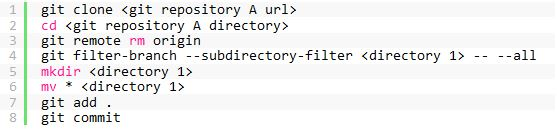
\includegraphics[width=0.50\textwidth]{Figures/PerpindahanFile}}
	\caption{PerpindahanFile}
	\label{PerpindahanFile}
\end{figure}

\chapter{Rename Operation}

\begin{references}{Ham62}
\bibitem[Kil76]{kilb}J. S. Kilby,
``Invention of the Integrated Circuit,'' {\it IEEE Trans. Electron Devices,}
{\bf ED-23,} 648 (1976).

\bibitem[Ham62]{hamm}R. W. Hamming,
                 {\it Numerical Methods for Scientists and 
                 Engineers}, Chapter N-1, McGraw-Hill, 
                 New York, 1962.

\bibitem[Hu86]{lee}J. Lee, K. Mayaram, and C. Hu, ``A Theoretical
               Study of Gate/Drain Offset in LDD MOSFETs''
                     {\it IEEE Electron Device Lett.,} {\bf EDL-7}(3). 152 
                     (1986).

\bibitem[Ber87]{berm}A. Berenbaum, 
B. W. Colbry, D.R. Ditzel, R. D Freeman, and 
K.J. O'Connor, ``A Pipelined 32b Microprocessor with 13 kb of Cache Memory,''
{it Int. Solid State Circuit Conf., Dig. Tech. Pap.,} p. 34 (1987).

\end{references}



%%%%%%%%%%%%%%%
%%  The default LaTeX Index
%%  Don't need to add any commands before \begin{document}
\printindex

%%%% Making an index
%% 
%% 1. Make index entries, don't leave any spaces so that they
%% will be sorted correctly.
%% 
%% \index{term}
%% \index{term!subterm}
%% \index{term!subterm!subsubterm}
%% 
%% 2. Run LaTeX several times to produce <filename>.idx
%% 
%% 3. On command line, type  makeindx <filename> which
%% will produce <filename>.ind 
%% 
%% 4. Type \printindex to make the index appear in your book.
%% 
%% 5. If you would like to edit <filename>.ind 
%% you may do so. See docs.pdf for more information.
%% 
%%%%%%%%%%%%%%%%%%%%%%%%%%%%%%

%%%%%%%%%%%%%% Making Multiple Indices %%%%%%%%%%%%%%%%
%% 1. 
%% \usepackage{multind}
%% \makeindex{book}
%% \makeindex{authors}
%% \begin{document}
%% 
%% 2.
%% % add index terms to your book, ie,
%% \index{book}{A term to go to the topic index}
%% \index{authors}{Put this author in the author index}
%% 
%% \index{book}{Cows}
%% \index{book}{Cows!Jersey}
%% \index{book}{Cows!Jersey!Brown}
%% 
%% \index{author}{Douglas Adams}
%% \index{author}{Boethius}
%% \index{author}{Mark Twain}
%% 
%% 3. On command line type 
%% makeindex topic 
%% makeindex authors
%% 
%% 4.
%% this is a Wiley command to make the indices print:
%% \multiprintindex{book}{Topic index}
%% \multiprintindex{authors}{Author index}

\end{document}

